% !TeX spellcheck = ru_RU
% !TEX root = vkr.tex

Данные, представимые в виде графов, встречаются повсеместно: при анализе компьютерных и социальных сетей, в биоинформатике и статическом анализе кода~\cite{gb_math}. Графы, возникающие в этих областях, могут содержать миллионы узлов и ребер, поэтому существует необходимость в высокопроизводительных инструментах анализа больших графов. В связи с этим многообещающей становится идея использования графических ускорителей общего назначения --- GPGPU. Существующие решения уже сейчас доказывают, что использование GPGPU может повысить производительность алгоритмов анализа графов~\cite{cusha}~\cite{mGPU}, однако ценой служит более сложная модель программирования~\cite{blast}. \\ Иным является подход к организации вычислений над графами, основанный на стандарте GraphBLAS~\cite{gb_math}, который определяет базовые примитивы для построения графовых алгоритмов в терминах линейной алгебры. Свойством такого подхода является способность оперировать богатым набором графов различных типов с помощью небольшого набора матричных операций над полукольцами. Например, умножение матрицы на вектор, как показано на рисунке~\ref{fig:bfs_step}, является шагом в алгоритме поиска в ширину. Решения, основанные на стандарте GraphBLAS, производительны, масштабируемы и имеют более дружественное API~\cite{sevengr}. Тем не менее на данный момент нет полноценных инструментов, реализующих стандарт GraphBLAS на графических процессорах общего назначения. Текущие реализации GraphBLAS на GPGPU (например, GraphBLAST~\cite{blast}) показывают, что использование GPGPU действительно может улучшить производительность инструментов такого рода, однако разработчики сталкиваются не только с проблемами, связанными с реализацией обобщенных операций на графических процессорах с помощью стандартных инструментов языка C++, но и с переносимостью решений, основанных на программно-аппаратной платформе CUDA.

\begin{figure}[h!]
    \centering
    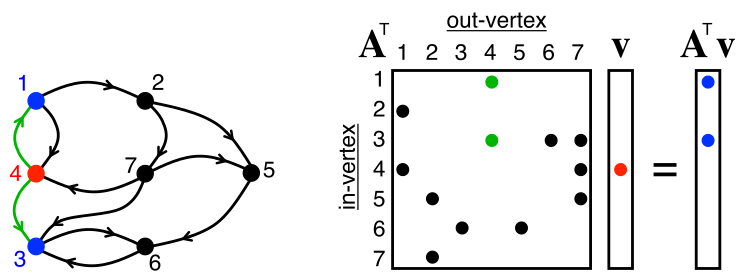
\includegraphics[width=0.6\linewidth]{pictures/MatrixBFS.png}
    \caption{Вычисление одного шага в алгоритме поиска в ширину\footnotemark}
    \label{fig:bfs_step}
\end{figure}

Одним из возможных подходов к реализации GraphBLAS на GPU является использование языка высокого уровня, а также библиотек, динамически транслирующих конструкции и объекты данного языка в низкоуровневый код, способный исполнятся на графическом процессоре видеокарты. Данный подход был опробован на прототипе GraphBLAS-sharp\footnote{Репозиторий библиотеки GraphBLAS-sharp: \url{https://github.com/YaccConstructor/GraphBLAS-sharp}. Дата посещения: 09.03.2022}, разработанном на кафедре системного программирования СПбГУ, который показал  жизнеспособность этой идеи. В качестве библиотеки для взаимодействия с OpenCL прототип использует библиотеку Brahma.FSharp, которая также разрабатывается на кафедре системного программирования СПбГУ. Библиотека позволяет использовать подмножество языка F\# для написания OpenCL ядер и предоставляет интерфейс для работы с ними. В ходе работы над прототипом GraphBLAS-sharp был выявлен ряд недостатков библиотеки \\ Brahma.FSharp, перечисленных ниже.
 
\begin{enumerate}
% \item Наличие больших накладных расходов на копирование данных между управляемой, неуправляемой и видеопамятью. (?)
\item Отсутствие атомарных операций для произвольных типов данных, что не позволяет реализовывать некоторые алгоритмы, которые могут оказаться лучше аналогов.
\item Отсутствие поддержки трансфера пользовательских типов данных
из управляемой памяти в видеопамять.
\item Отсутствие возможности вручную управлять выделением памяти на OpenCL устройстве.
\item Отсутствие возможности исполнения нескольких OpenCL ядер параллельно.
\end{enumerate}

\footnotetext{GraphBLAS [Электронный ресурс] // Википедия. Свободная энциклопедия. – URL: \url{https://en.wikipedia.org/wiki/GraphBLAS} (дата обращения: 01.01.2022).}
